\section{Biological Nanopores}

Biological nanopores are small perforations in the bi lipid membrane, created by a pore
forming protein.  These proteins are toxins
produced by bacteria, as means of killing targeted cells. They work by perforating
the cell membrane of a cell, of which the contents is spilled into the
environment though osmoses, thereby killing the cell.

The small scale of these protein structures, a few nanometers across,


due to their small scale ideal for spectroscopy.

short introduction to their structural.

should be noted that also solid state nano pores exist poking hole in semi conductor.
Prescission is much less so currently bio pores are better. Interesting future.


\subsection{$\alpha$-Hemolysin ($\alpha$ HL)}
\begin{figure}[h!]
  \centering
  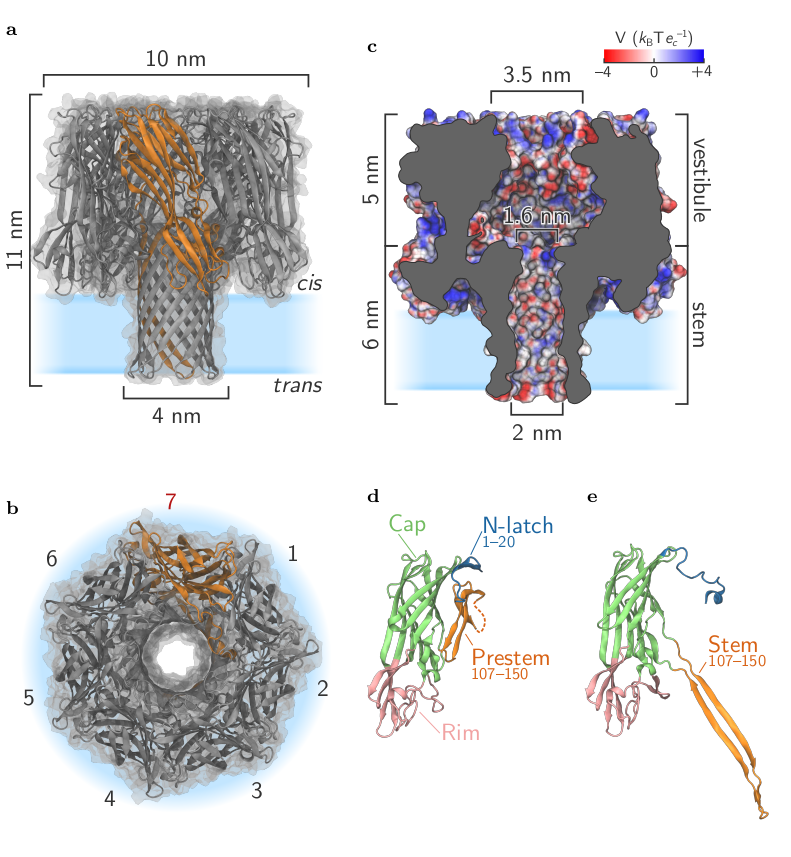
\includegraphics[width=0.5\linewidth]{Figures/alpha-hemolysin.png}
  \caption{write caption}
  \label{adsf}
\end{figure}


\subsection{Cytolysin A (ClyA)}
\begin{figure}[h!]
  \centering
  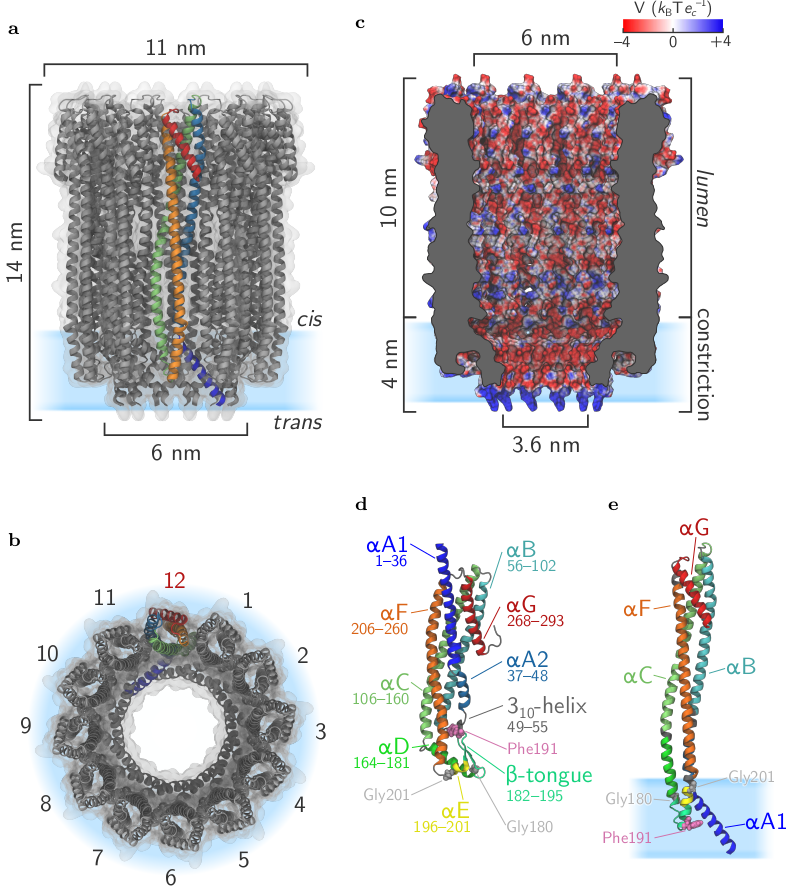
\includegraphics[width=0.5\linewidth]{Figures/cytolysinA.png}
  \caption{write caption}
  \label{adassf}
\end{figure}
\subsection{Ionic current spectroscopy}

It should be noted that besides these biological nanopores, there are also solid state
nanopore under development. nog niet zo goed als bio pores, maar hebben het voordeel dat
ze heel goed afgesteld kunnen worden -> dit is de toekomst!
